\documentclass[preprint,12pt]{elsarticle}

\usepackage[T1]{fontenc}
\usepackage{amsmath}
\usepackage{amssymb}
\usepackage{booktabs}
\usepackage{graphicx}
\usepackage{xspace}

\graphicspath{{figures/}{../../data/}}

\journal{Physics Letters B}

\newcommand{\snn}{\sqrt{s_{NN}}\xspace}
\newcommand{\mub}{\mu_B\xspace}
\newcommand{\mus}{\mu_S\xspace}
\newcommand{\muq}{\mu_Q\xspace}
\newcommand{\tch}{T_{\rm ch}\xspace}
\newcommand{\dndy}{dN/dy\xspace}
\newcommand{\chisqndf}{\chi^2/{\rm ndf}\xspace}
\newcommand{\particlesSCE}{$p$, $K^-$, $K^0_S$, $\Lambda$, $\Xi^-$, $\phi$}
\newcommand{\particlesGCEFull}{$\pi^\pm$, $K^\pm$, $p$, $\bar p$, $\Lambda$, $\bar\Lambda$, $\Xi^-$, $\bar\Xi^+$, $\phi$}
\newcommand{\particlesGCEPartial}{$\pi^\pm$, $K^\pm$, $p$, $\bar p$, $\Lambda$, $\bar\Lambda$, $\Xi^-$, $\bar\Xi^+$}

\begin{document}

\begin{frontmatter}

\title{Chemical freeze-out from a THERMUS analysis of STAR hadron yields from $\sqrt{s_{NN}}=3$ to $200$ GeV}

\author[inst1]{First Author}
\author[inst1]{Second Author}
\author[inst2]{Third Author}
\address[inst1]{Affiliation 1, City, Country}
\address[inst2]{Affiliation 2, City, Country}

\begin{abstract}
We analyze STAR midrapidity hadron yields in central Au+Au collisions from $\sqrt{s_{NN}}=3$ to $200$ GeV.
At $\sqrt{s_{NN}}=7.7$--$200$ GeV, grand-canonical THERMUS fits to $\pi^\pm$, $K^\pm$, $p(\bar p)$, $\Lambda(\bar\Lambda)$, $\Xi(\bar\Xi)$, and $\phi$ yields give a smooth chemical freeze-out trajectory with $T_{\rm ch}$ increasing from $146.1\pm2.8$ MeV at $7.7$ GeV to $166.2\pm3.3$ MeV at $200$ GeV, while $\mu_B$ decreases from $407\pm14$ MeV to $27\pm12$ MeV.
The same treatment cannot be continued smoothly to $\sqrt{s_{NN}}=3$ GeV.
Using a strangeness-canonical ensemble for the measured $p$, $K^-$, $K^0_S$, $\Lambda$, $\Xi^-$, and $\phi$ yields at 3 GeV, we obtain $T_{\rm ch}=81.7\pm4.5$ MeV, $\mu_B=751\pm16$ MeV, and a strangeness correlation radius $R_C=3.69\pm0.87$ fm.
The result indicates a sharp change of the chemical freeze-out conditions between 3 and 7.7 GeV and demonstrates that canonical strangeness conservation is essential for describing strange-hadron production in the high-baryon-density regime.
\end{abstract}

\begin{keyword}
chemical freeze-out \sep strangeness canonical ensemble \sep THERMUS \sep STAR \sep beam energy scan \sep heavy-ion collisions
\end{keyword}

\end{frontmatter}

\section{Introduction}

Integrated hadron yields in relativistic heavy-ion collisions encode the chemical composition of the fireball at the stage where inelastic reactions cease.
Statistical hadronization models have therefore become a standard tool for determining the chemical freeze-out temperature and chemical potentials over a broad range of collision energies \cite{Andronic2018Nature,Wheaton2009THERMUS}.
The RHIC Beam Energy Scan provides a particularly useful dataset because the same experiment measured identified hadrons over a large range of baryon chemical potential.
Existing STAR analyses established freeze-out parameters at $\sqrt{s_{NN}}=7.7$--$39$ GeV from light hadrons and strange hadrons \cite{STARBulk2017,STARStrange2020}, with complementary high-energy information at 62.4 and 200 GeV \cite{STARIdentified2009,STARStrange2007,STARStrange2011}.

The recent fixed-target and collider measurements at $\sqrt{s_{NN}}=3$ GeV extend this program into a much higher baryon-density region.
At this energy, STAR has measured protons and light nuclei \cite{STARLightNuclei3GeV}, $K^-$, $\phi$, and $\Xi^-$ \cite{STARKPhiXi3GeV}, and $K^0_S$ and $\Lambda$ production \cite{STARKsLambda3GeV}.
The 3 GeV system differs qualitatively from the higher-energy BES-I regime: antibaryon yields are strongly suppressed, the strange-particle phase space is sparse, and exact conservation of strangeness over a finite correlation volume can substantially affect strange-hadron yields.
In this Letter we apply a common THERMUS-based workflow to the available STAR data at 3 GeV and 7.7--200 GeV, quantify the extracted freeze-out parameters, and compare grand-canonical and strangeness-canonical descriptions in the low-energy region.

\section{Data and model setup}

THERMUS implements a statistical hadron-resonance gas calculation in which hadron yields are fixed by a chemical freeze-out temperature, chemical potentials associated with conserved charges, and a fireball volume \cite{Wheaton2009THERMUS}.
For a particle species $i$, the calculated midrapidity yield can be written schematically as
\begin{equation}
\frac{dN_i}{dy} = V \, n_i(T_{\rm ch},\mu_B,\mu_S,\mu_Q,\gamma_S),
\end{equation}
where $n_i$ includes the thermal density and the resonance decay feed-down implemented in THERMUS.
In this work the volume is represented by the radius parameter $R$ and the strangeness saturation parameter is fixed to $\gamma_S=1$.

For the $\sqrt{s_{NN}}=7.7$--200 GeV data we use the grand-canonical ensemble (GCE).
In the GCE, baryon number, strangeness, and electric charge are conserved on average through the chemical potentials $\mu_B$, $\mu_S$, and $\mu_Q$.
This approximation is appropriate when the relevant conserved charges are abundantly produced in the fitted rapidity interval, so that canonical suppression effects are small compared with the experimental and model uncertainties.
At $\sqrt{s_{NN}}=3$ GeV the strange-particle multiplicities are much smaller, and exact local strangeness conservation becomes important.
We therefore use the strangeness-canonical ensemble (SCE), in which the total strangeness is fixed exactly inside a correlation volume $V_C=4\pi R_C^3/3$, while baryon number and electric charge remain grand canonical.
The resulting canonical factors suppress open-strangeness hadrons in a way that depends on their strangeness content and on $R_C$; hidden-strangeness particles such as the $\phi$ are not suppressed in the same manner.

The high-energy fits use midrapidity yields for central Au+Au collisions at $\sqrt{s_{NN}}=7.7$, 11.5, 19.6, 27, 39, 62.4, and 200 GeV.
The fitted species are $\pi^\pm$, $K^\pm$, $p$, $\bar p$, $\Lambda$, $\bar\Lambda$, $\Xi^-$, $\bar\Xi^+$, and $\phi$ where available.
The 62.4 GeV point has a smaller input set and should be interpreted with correspondingly larger sensitivity to the selected data.
The proton and antiproton inputs are corrected for weak $\Lambda$ and $\bar\Lambda$ feed-down using the branching fraction 0.639.
For these energies we use the grand-canonical ensemble with free parameters $\tch$, $\mub$, $\mus$, and a radius parameter $R$; $\gamma_S$ is fixed to unity.

At $\sqrt{s_{NN}}=3$ GeV we fit the measured $p$, $K^-$, $K^0_S$, $\Lambda$, $\Xi^-$, and $\phi$ yields.
The sparse antiparticle sector and the observed hierarchy of strange-hadron yields motivate a mixed ensemble in which strangeness is conserved canonically in a correlation volume with radius $R_C$, while baryon number and electric charge are treated grand canonically.
The 3 GeV fit parameters are $\tch$, $\mub$, $\muq$, $R_C$, and $R$, again with $\gamma_S=1$.
The electric-charge constraint uses the Au participant value $B/(2Q)=1.246835$.

\section{Results}

Figure~\ref{fig:freezeout} summarizes the extracted THERMUS parameters as a function of collision energy, and Fig.~\ref{fig:freezeouttrajectory} shows the corresponding freeze-out trajectory in the $(\mub,\tch)$ plane.
The grand-canonical fits above 7.7 GeV follow the expected monotonic decrease of $\mub$ with increasing beam energy and a gradual saturation of $\tch$ near 160--166 MeV.
The numerical values are listed in Table~\ref{tab:fitparams}, and the particle species included in the fits are summarized in Table~\ref{tab:fitparticles}.
For all high-energy points except 62.4 GeV, the fit quality is $\chisqndf\simeq1.0$--1.6.
The 62.4 GeV fit gives $\chisqndf=4.26$, driven by the reduced and heterogeneous input set; it is retained in the systematics but should not be overinterpreted as a precision freeze-out point.

\begin{figure}[t]
\centering
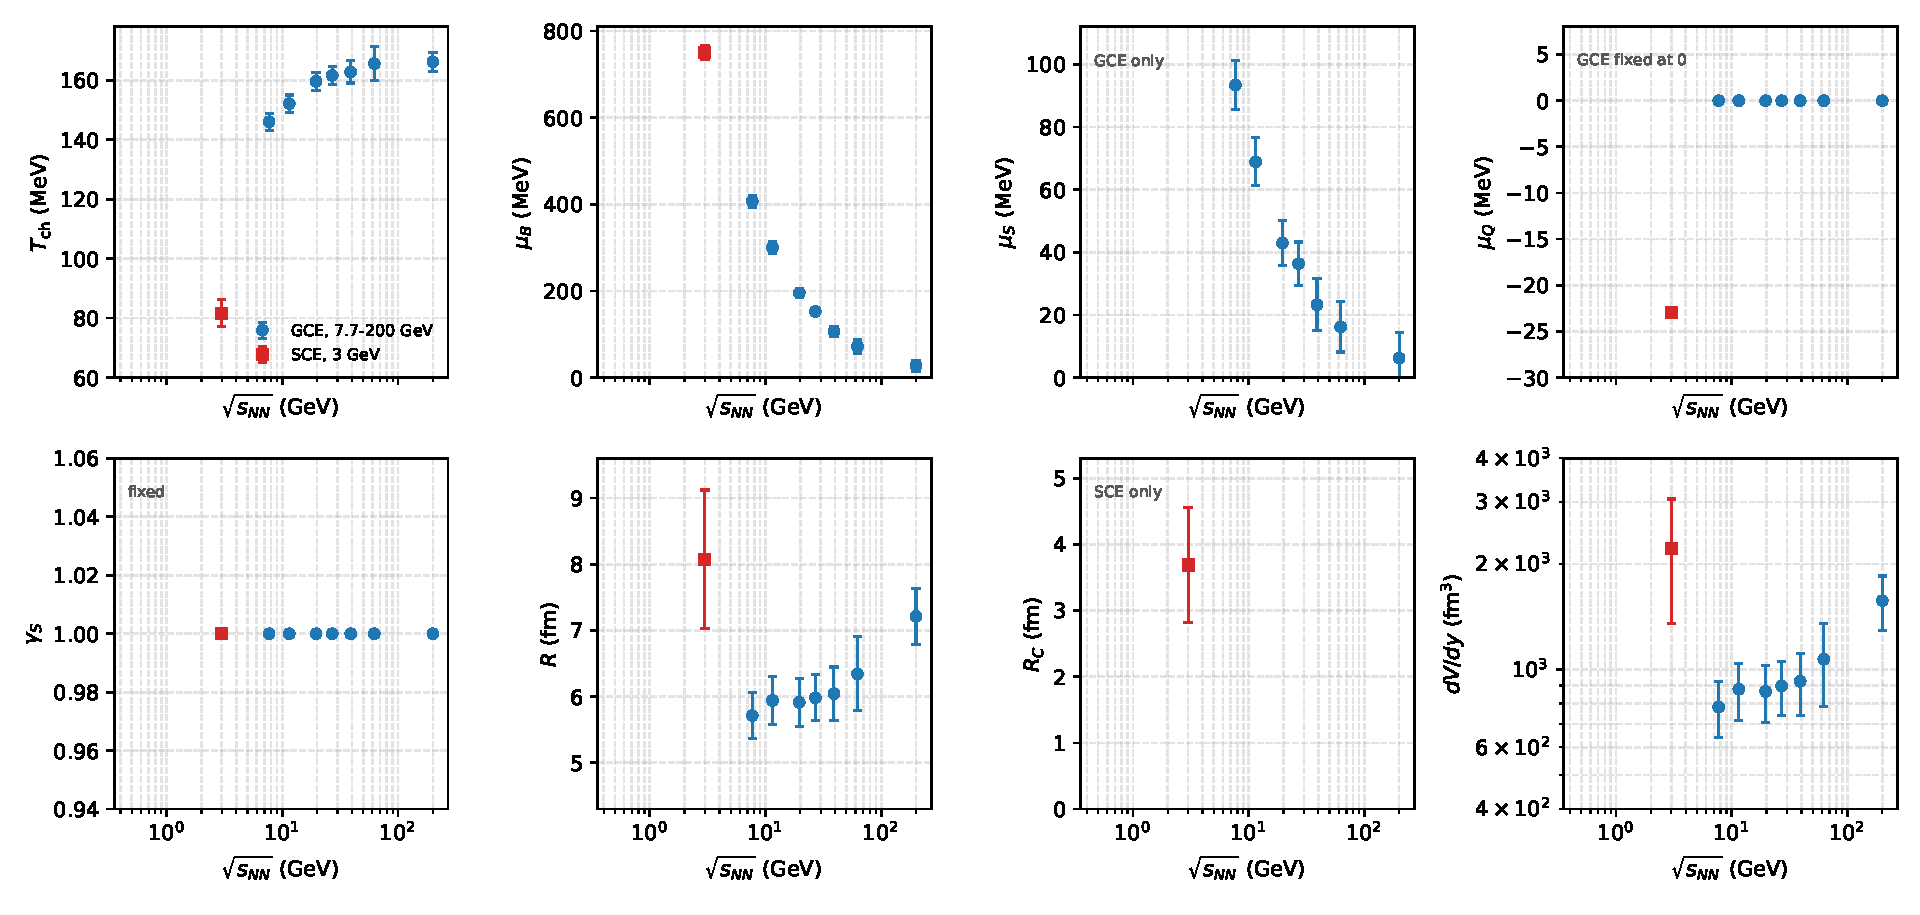
\includegraphics[width=\linewidth]{freezeout_summary.pdf}
\caption{THERMUS parameters from the STAR Au+Au fits versus collision energy.
The panels show $\tch$, $\mub$, $\mus$, $\muq$, $\gamma_S$, the fireball radius $R$, the strangeness-canonical correlation radius $R_C$, and the derived midrapidity volume $dV/dy=4\pi R^3/3$.
Blue circles are grand-canonical fits at $\sqrt{s_{NN}}=7.7$--200 GeV; the red square is the strangeness-canonical 3 GeV fit.
For the GCE fits, $\muq$ is fixed to zero and $R_C$ is not used.
For the SCE fit, strangeness is conserved exactly rather than through $\mus$.
The parameter $\gamma_S$ is fixed to unity in all fits.}
\label{fig:freezeout}
\end{figure}

\begin{figure}[t]
\centering
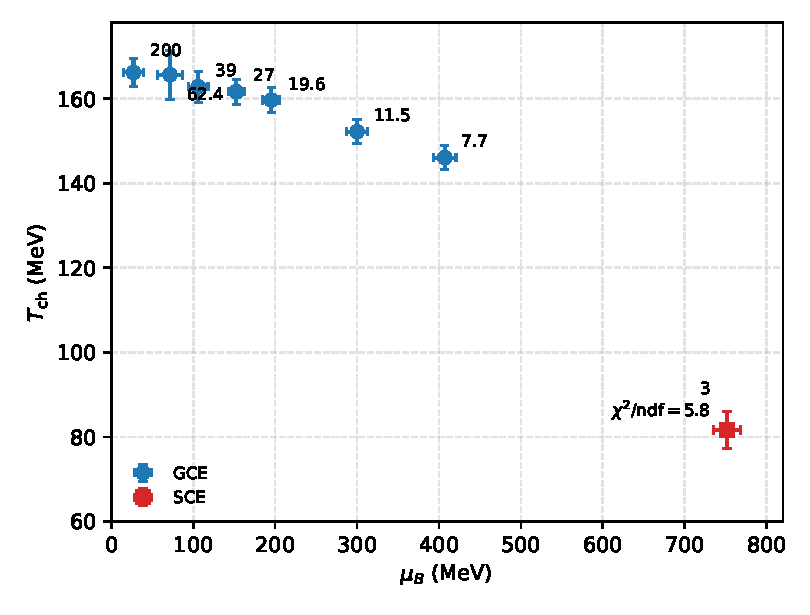
\includegraphics[width=0.72\linewidth]{freezeout_t_vs_mub.pdf}
\caption{Chemical freeze-out trajectory in the $(\mub,\tch)$ plane from the THERMUS fits.
Point labels indicate $\sqrt{s_{NN}}$ in GeV.
The 3 GeV strangeness-canonical fit lies well separated from the grand-canonical 7.7--200 GeV trajectory.}
\label{fig:freezeouttrajectory}
\end{figure}

\begin{table}[t]
\centering
\caption{THERMUS fit parameters for STAR Au+Au data compared with published STAR chemical-freeze-out values where available \cite{STARBulk2017,STARStrange2011}. Uncertainties are fit uncertainties.}
\label{tab:fitparams}
\small
\resizebox{\linewidth}{!}{%
\begin{tabular}{@{}cccccccc@{}}
\toprule
$\sqrt{s_{NN}}$ (GeV) & Ensemble & $N_{\rm data}$ & $\tch$ & STAR $\tch$ & $\mub$ & STAR $\mub$ & $\chisqndf$ \\
\multicolumn{3}{c}{} & \multicolumn{2}{c}{(MeV)} & \multicolumn{2}{c}{(MeV)} & \\
\midrule
3.0   & SCE & 6  & $81.7\pm4.5$  & --           & $751\pm16$ & --          & 5.81 \\
7.7   & GCE & 11 & $146.1\pm2.8$ & $144\pm3$   & $407\pm14$ & $400\pm13$ & 1.16 \\
11.5  & GCE & 11 & $152.2\pm2.9$ & $151\pm3$   & $300\pm13$ & $292\pm13$ & 1.38 \\
19.6  & GCE & 11 & $159.7\pm3.0$ & $158\pm3$   & $195\pm10$ & $196\pm10$ & 1.56 \\
27.0  & GCE & 11 & $161.6\pm2.9$ & $160\pm3$   & $153\pm10$ & $152\pm9$  & 1.16 \\
39.0  & GCE & 11 & $162.8\pm3.7$ & $160\pm4$   & $106\pm12$ & $105\pm11$ & 1.05 \\
62.4  & GCE & 8  & $165.6\pm5.8$ & $162\pm6$   & $72\pm15$  & $69\pm7$   & 4.26 \\
200   & GCE & 11 & $166.2\pm3.3$ & $165\pm6$   & $27\pm12$  & $26\pm7$   & 1.46 \\
\bottomrule
\end{tabular}
}
\end{table}

\begin{table}[t]
\centering
\caption{Particle species included in the THERMUS fits.}
\label{tab:fitparticles}
\small
\begin{tabular}{@{}p{0.22\linewidth}cp{0.56\linewidth}@{}}
\toprule
$\sqrt{s_{NN}}$ (GeV) & Ensemble & Fitted particles \\
\midrule
3.0 & SCE & \particlesSCE \\
7.7--39.0, 200 & GCE & \particlesGCEFull \\
62.4 & GCE & \particlesGCEPartial \\
\bottomrule
\end{tabular}
\end{table}

The extracted 3 GeV point lies far below an extrapolation of the high-energy freeze-out temperature while reaching a much larger baryon chemical potential.
The strangeness-canonical fit gives $R_C=3.69\pm0.87$ fm and $R=8.08\pm1.05$ fm, corresponding to $dV/dy=2207\pm857$ fm$^3$.
The fit quality, $\chisqndf=5.81$, is not at the level of the high-energy GCE fits.
This tension is physically informative rather than merely technical: no single equilibrium parameter set describes all 3 GeV strange-hadron yields with the same accuracy achieved at higher energies.
The largest residuals arise from the multistrange and hidden-strangeness sector, where production can be sensitive to canonical suppression, hadronic rescattering, and associated-production dynamics.

\begin{figure}[t]
\centering
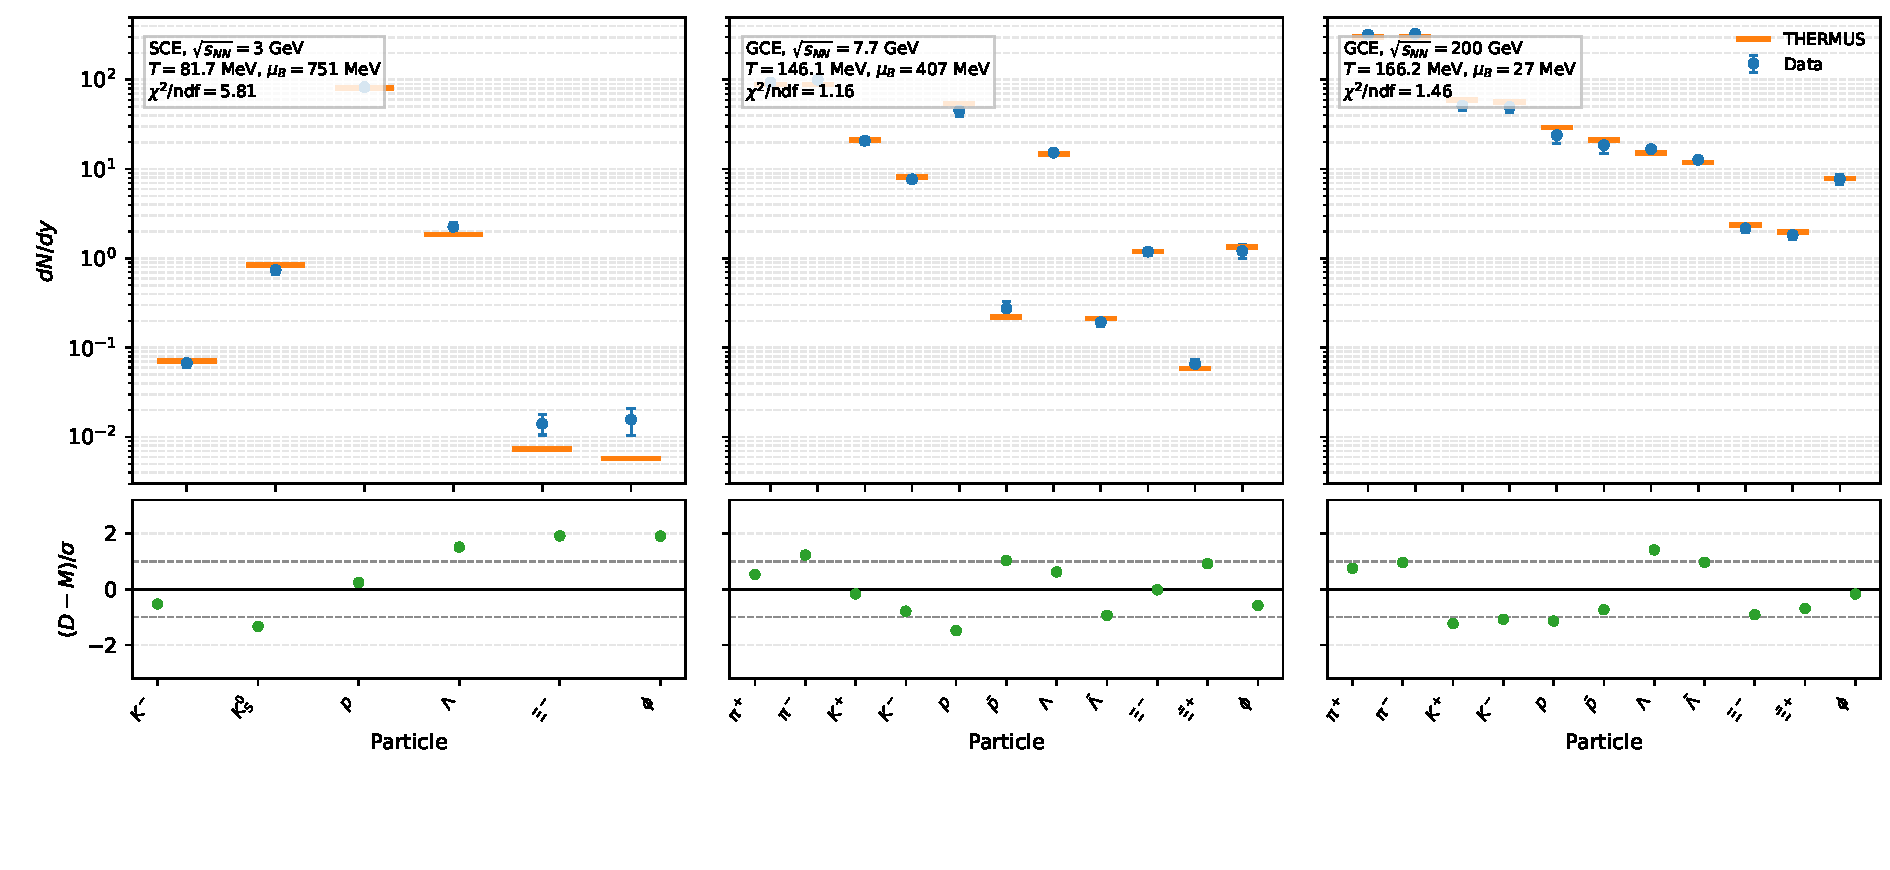
\includegraphics[width=\linewidth]{yield_comparison_selected_energies.pdf}
\caption{Representative yield comparisons entering the THERMUS analysis.
The panels show $\sqrt{s_{NN}}=3.0$ GeV SCE, 7.7 GeV GCE, and 200 GeV GCE fits.
Upper panels compare fitted STAR yields with the corresponding THERMUS fit values; lower panels show residuals $(D-M)/\sigma$.}
\label{fig:yieldfits}
\end{figure}

Figure~\ref{fig:yieldfits} shows direct data-to-fit comparisons at representative low, intermediate, and high collision energies.
The 7.7 and 200 GeV GCE fits describe the fitted yields at the level expected from their $\chisqndf$ values, while the 3 GeV SCE comparison makes the remaining tension in the multistrange and hidden-strangeness sector explicit.

Figure~\ref{fig:yields} compares the measured excitation functions with the THERMUS calculations.
The high-energy GCE calculation captures the dominant energy trends of pions, kaons, protons, $\Lambda$, $\Xi$, and $\phi$ over nearly two orders of magnitude in $\snn$.
No interpolated model curve is drawn between 3 and 7.7 GeV.
Instead, the 3 GeV SCE fit is shown only as horizontal bars at the fitted particle yields.
The strangeness-canonical treatment reduces the open-strangeness yields relative to a naive grand-canonical continuation and improves the qualitative description of the low-energy strange sector.
Hidden strangeness, represented by $\phi$, is not canonically suppressed in the same way, providing a useful discriminator between canonical suppression and a global reduction of all strange-particle production.

\begin{figure}[t]
\centering
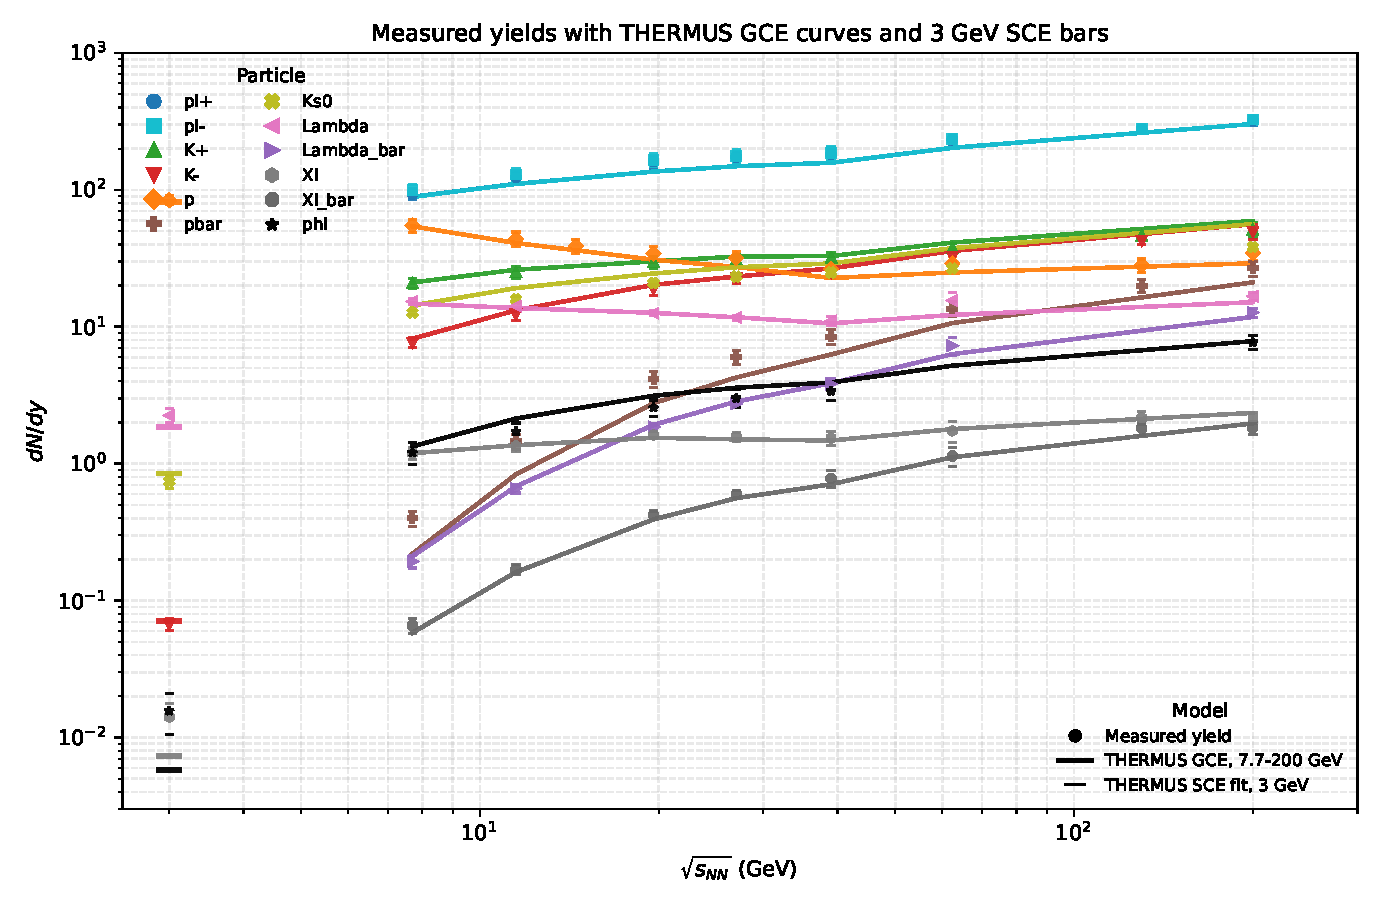
\includegraphics[width=\linewidth]{strange_hadron_model_comparison_triptych.pdf}
\caption{Measured hadron yields compared with THERMUS calculations.
The symbols show STAR data used in the fit or model comparison.
Solid curves show the grand-canonical THERMUS calculation for $\sqrt{s_{NN}}\geq7.7$ GeV; horizontal bars at 3 GeV show the strangeness-canonical THERMUS fit values.}
\label{fig:yields}
\end{figure}

\section{Discussion}

The discontinuity between the 3 GeV strangeness-canonical point and the 7.7--200 GeV grand-canonical trajectory should be read as evidence that the chemical composition at 3 GeV is controlled by additional constraints and dynamics.
The extracted $\tch$ of about 82 MeV is much lower than the 7.7 GeV value of about 146 MeV, while $\mub$ increases by roughly 340 MeV.
This behavior is consistent with the expectation that the 3 GeV collision system is baryon rich and hadron dominated.
It is also consistent with other STAR observations at 3 GeV that point to strong baryonic interactions in the produced medium.

The 3 GeV panel of Fig.~\ref{fig:yieldfits} isolates the low-energy fit quality.
For the particles with available 3 GeV measurements, the strangeness-canonical fit values follow the measured hierarchy more closely than a naive GCE continuation.
The improvement is largest for open-strangeness hadrons carrying one or more strange quarks.
However, the remaining residuals and the high 3 GeV $\chisqndf$ show that canonical suppression alone is not a complete microscopic explanation.
The sparse species set, different rapidity coverages, and possible non-equilibrium production channels limit the precision with which a unique freeze-out point can be assigned at this energy.

\section{Conclusions}

We have constructed a common THERMUS analysis of STAR hadron yields from $\sqrt{s_{NN}}=3$ to 200 GeV.
Grand-canonical fits at 7.7--200 GeV reproduce the measured central-yield systematics with a smooth freeze-out trajectory and fit qualities near unity for most energies.
At 3 GeV, a strangeness-canonical description is required and yields a much lower chemical freeze-out temperature, $T_{\rm ch}=81.7\pm4.5$ MeV, and a high baryon chemical potential, $\mu_B=751\pm16$ MeV.
The extracted strangeness correlation radius is $R_C=3.69\pm0.87$ fm.
The result demonstrates a qualitative change in the chemistry of strange hadrons between $\sqrt{s_{NN}}=3$ and 7.7 GeV.
Future simultaneous fits including additional pion, kaon, light-nuclei, and hypernuclei yields at the same centrality and rapidity will be essential for separating canonical conservation effects from hadronic production dynamics in the high-baryon-density regime.

\section*{Acknowledgements}

Add funding and collaboration acknowledgements here.

\section*{Declaration of competing interest}

The authors declare no known competing financial interests or personal relationships that could have appeared to influence the work reported in this paper.

\section*{Data availability}

The analysis inputs and scripts used to prepare the tables and figures are stored in the accompanying repository. The experimental inputs are taken from the cited STAR publications and the corresponding HEPData records where available.

\section*{Declaration of generative AI and AI-assisted technologies}

During preparation of this manuscript draft, AI-assisted text generation was used to organize and edit the prose. The scientific content, numerical results, citations, and conclusions require verification and approval by the authors before submission.

\bibliographystyle{elsarticle-num}
\bibliography{references}

\end{document}
